\section{Meridional propagation of GWs excited by tropopause depressions}
\label{sec:results3D}

Eventually eight full 3D simulations were conducted to investigate the effect of a tilted TD and horizontal wind shear on the meridional propagation of GWs.
Three simulations without horizontal shear an


Add another simulation with a stronger PNJ and stronger horizontal shear to observe 
\subsection{Effects of TD orientation in atmosphere}
% no meridional shear


\subsection{Variations of the TD's zonal width and its effect on the meridional propagation of GWs}

extrinsic frequency is conserved along the ray. Is 0 for stationary mountain waves.

intrinsic frequency = 




\subsection{The impact of rotating the TD with respect to the zonal}
% no meridional shear

- Wavelet analysis described earlier

- 

\begin{figure*}[]
    \centering
    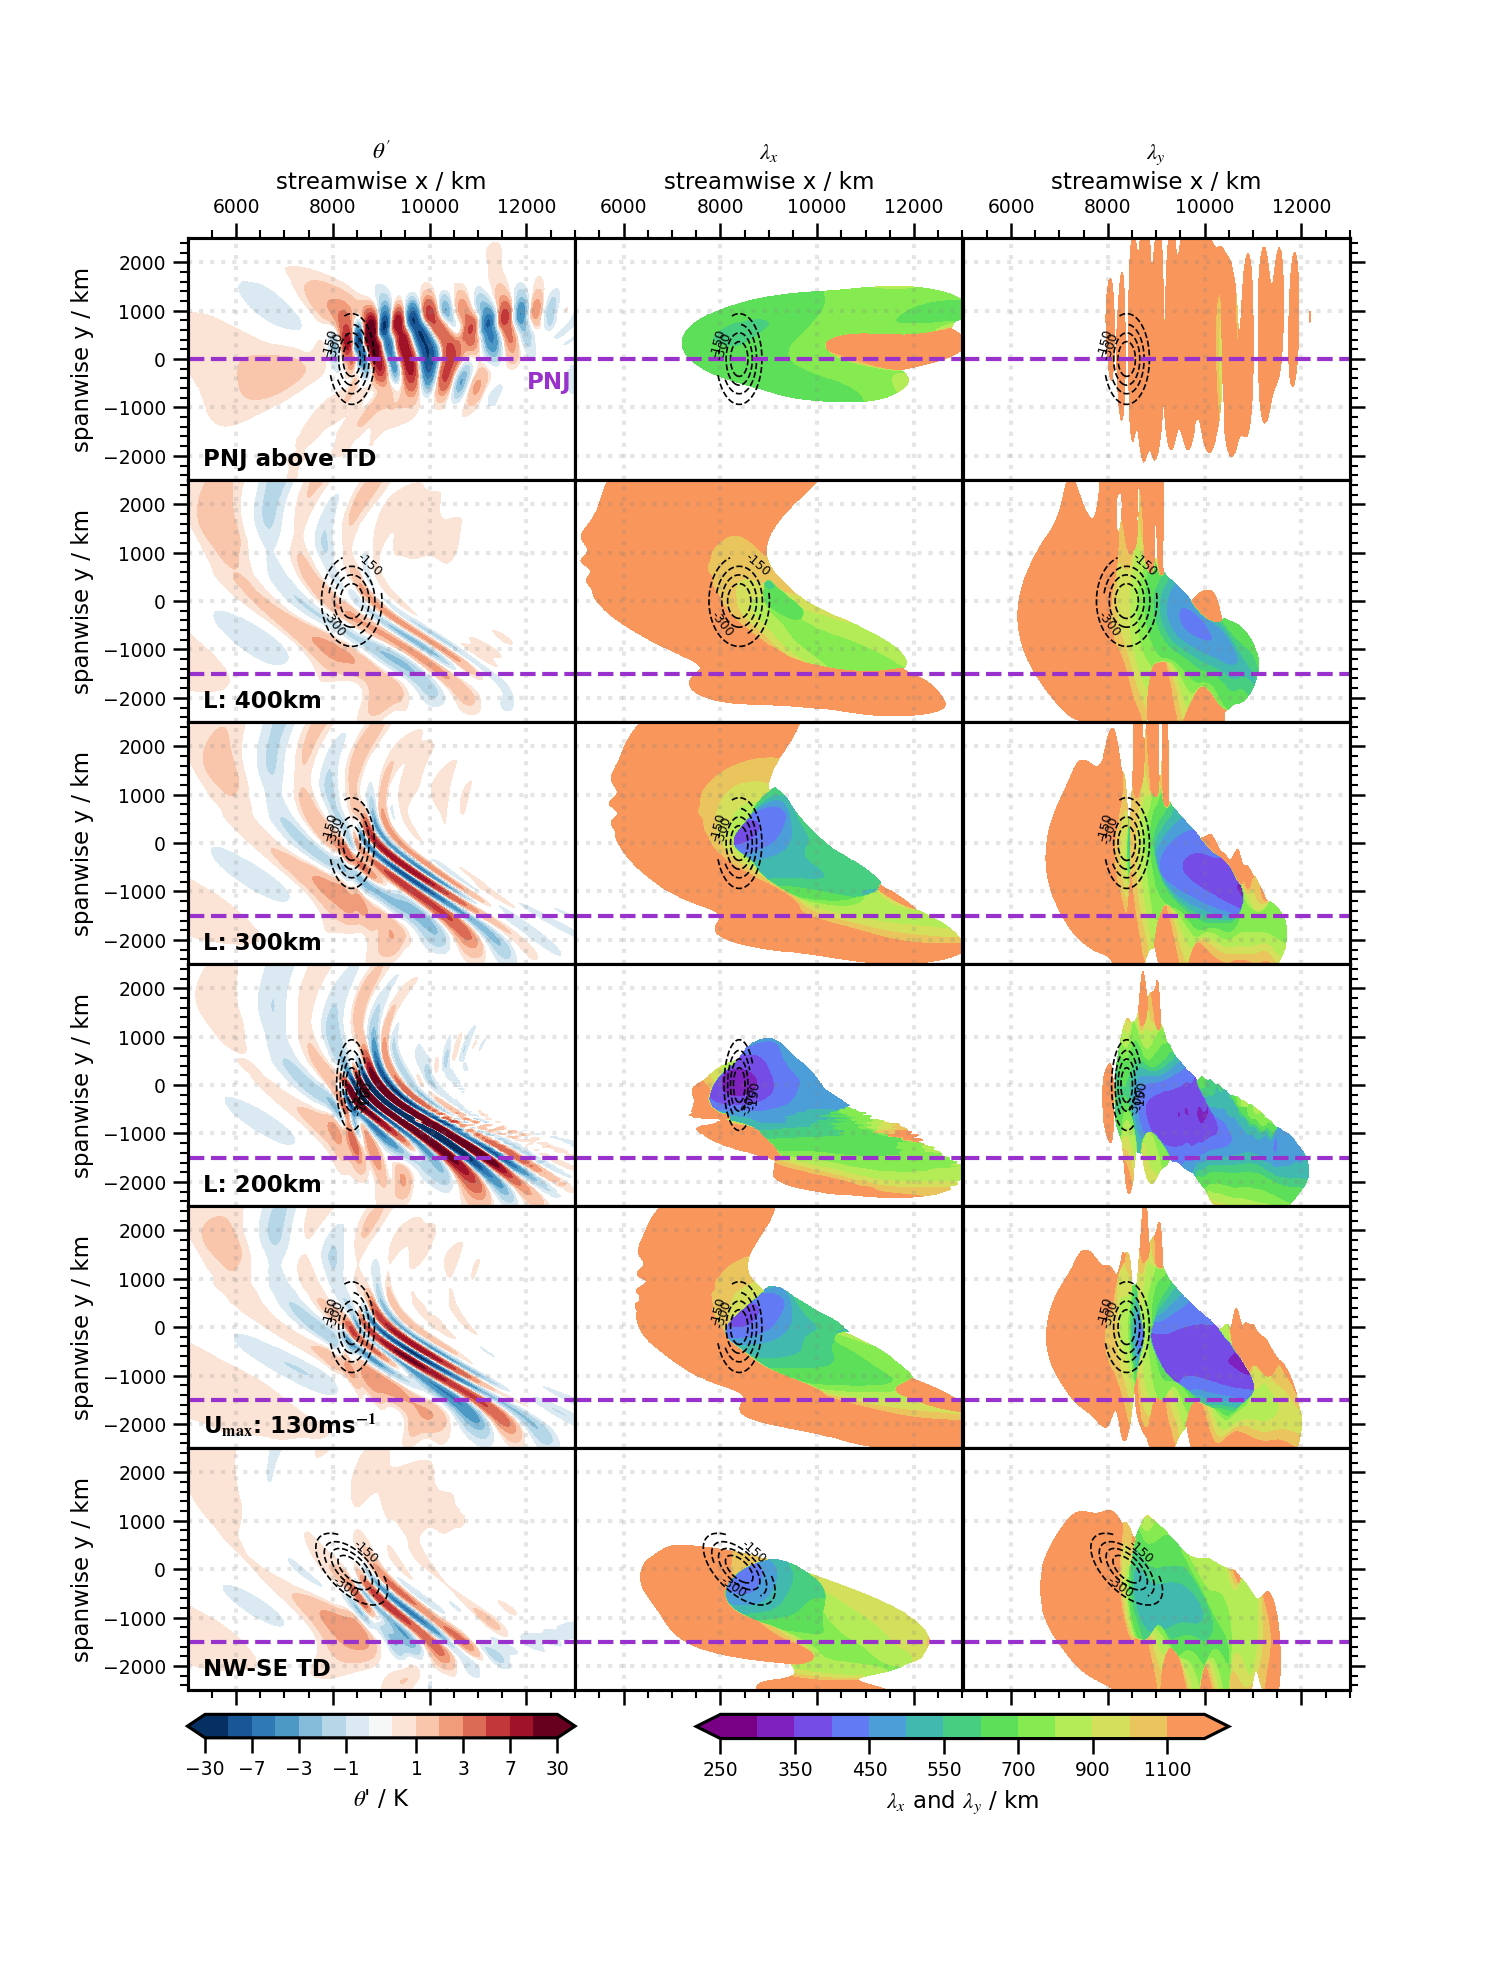
\includegraphics[width=0.99\textwidth]{figures_3D/waveletAna_dudy.png}
    \caption{Horizontal cross sections at 40km above the tropopause for five simulations with horizontal and meridional shear in a barotropic environment. Shown are $\theta$', $\lambda_x$ and $\lambda_y$ at 72h into the simulation. Dominant zonal and meridional wavelengths for each grid point are determined from wavelet analysis.}
    \label{fig:waveletAna_dudy}
\end{figure*}


\subsection{Momentum fluxes from a simulation-based and observational perspective}

MF$_x$ MF$_y$ can be calculated directly from wind perturbations ($u'$, $v'$,$w'$) provided by the numerical simulation with the EULAG model. However, most satellite or ground-based observations measure temperature perturbations without further information on the corresponding wind (e.g. \cite{hindley_gravity_2019}, \cite{kaifler_compact_2021}, \cite{wu_satellite_1996}). For 2D Lidar observations these measurements usually aren't sufficient to derive horizontal momentum fluxes without additional information or assumptions for horizontal wavelengths. In the case of three dimensional datasets, as analysed by \textcite{hindley_18year_2020} (satellite observations), the determination of momentum fluxes is possible under the midfrequency approximation. This analysis follows \textcite{ern...} and combines the calculation of the potential energy (equation PE) with a three dimensional spectral analysis to obtain corresponding wavenumbers. Zonal and meridional momentum fluxes are 

\begin{equation}
    (\mathrm{MF}_x, \mathrm{MF}_y) = \frac{\rho}{2} (\frac{g}{N})^2 (\frac{T'}{\bar{T}})^2 (\frac{k}{m},\frac{l}{m})
\end{equation}

% with $\rho$ being the density, $g$ the gravitational acceleration, N the Brunt‐Väisälä frequency, $T'$ and $\bar{T}$ temperature perturbations and background temperature respectively and $k,l,m$ are zonal, meridional and vertical wavenumbers (\cite{ern}). This relation is valid for hydrostatic and nonrotational GWs with an intrinsic frequency in the range $f \ll \hat{\omega} \ll N$, where $f$ is the inertial frequency (e.g., Fritts & Alexander, 2003).

Maybe it makes sense that MFx via wavelet analysis is smaller, because it collapses contribution to a single frequency

\begin{figure*}[]
    \centering
    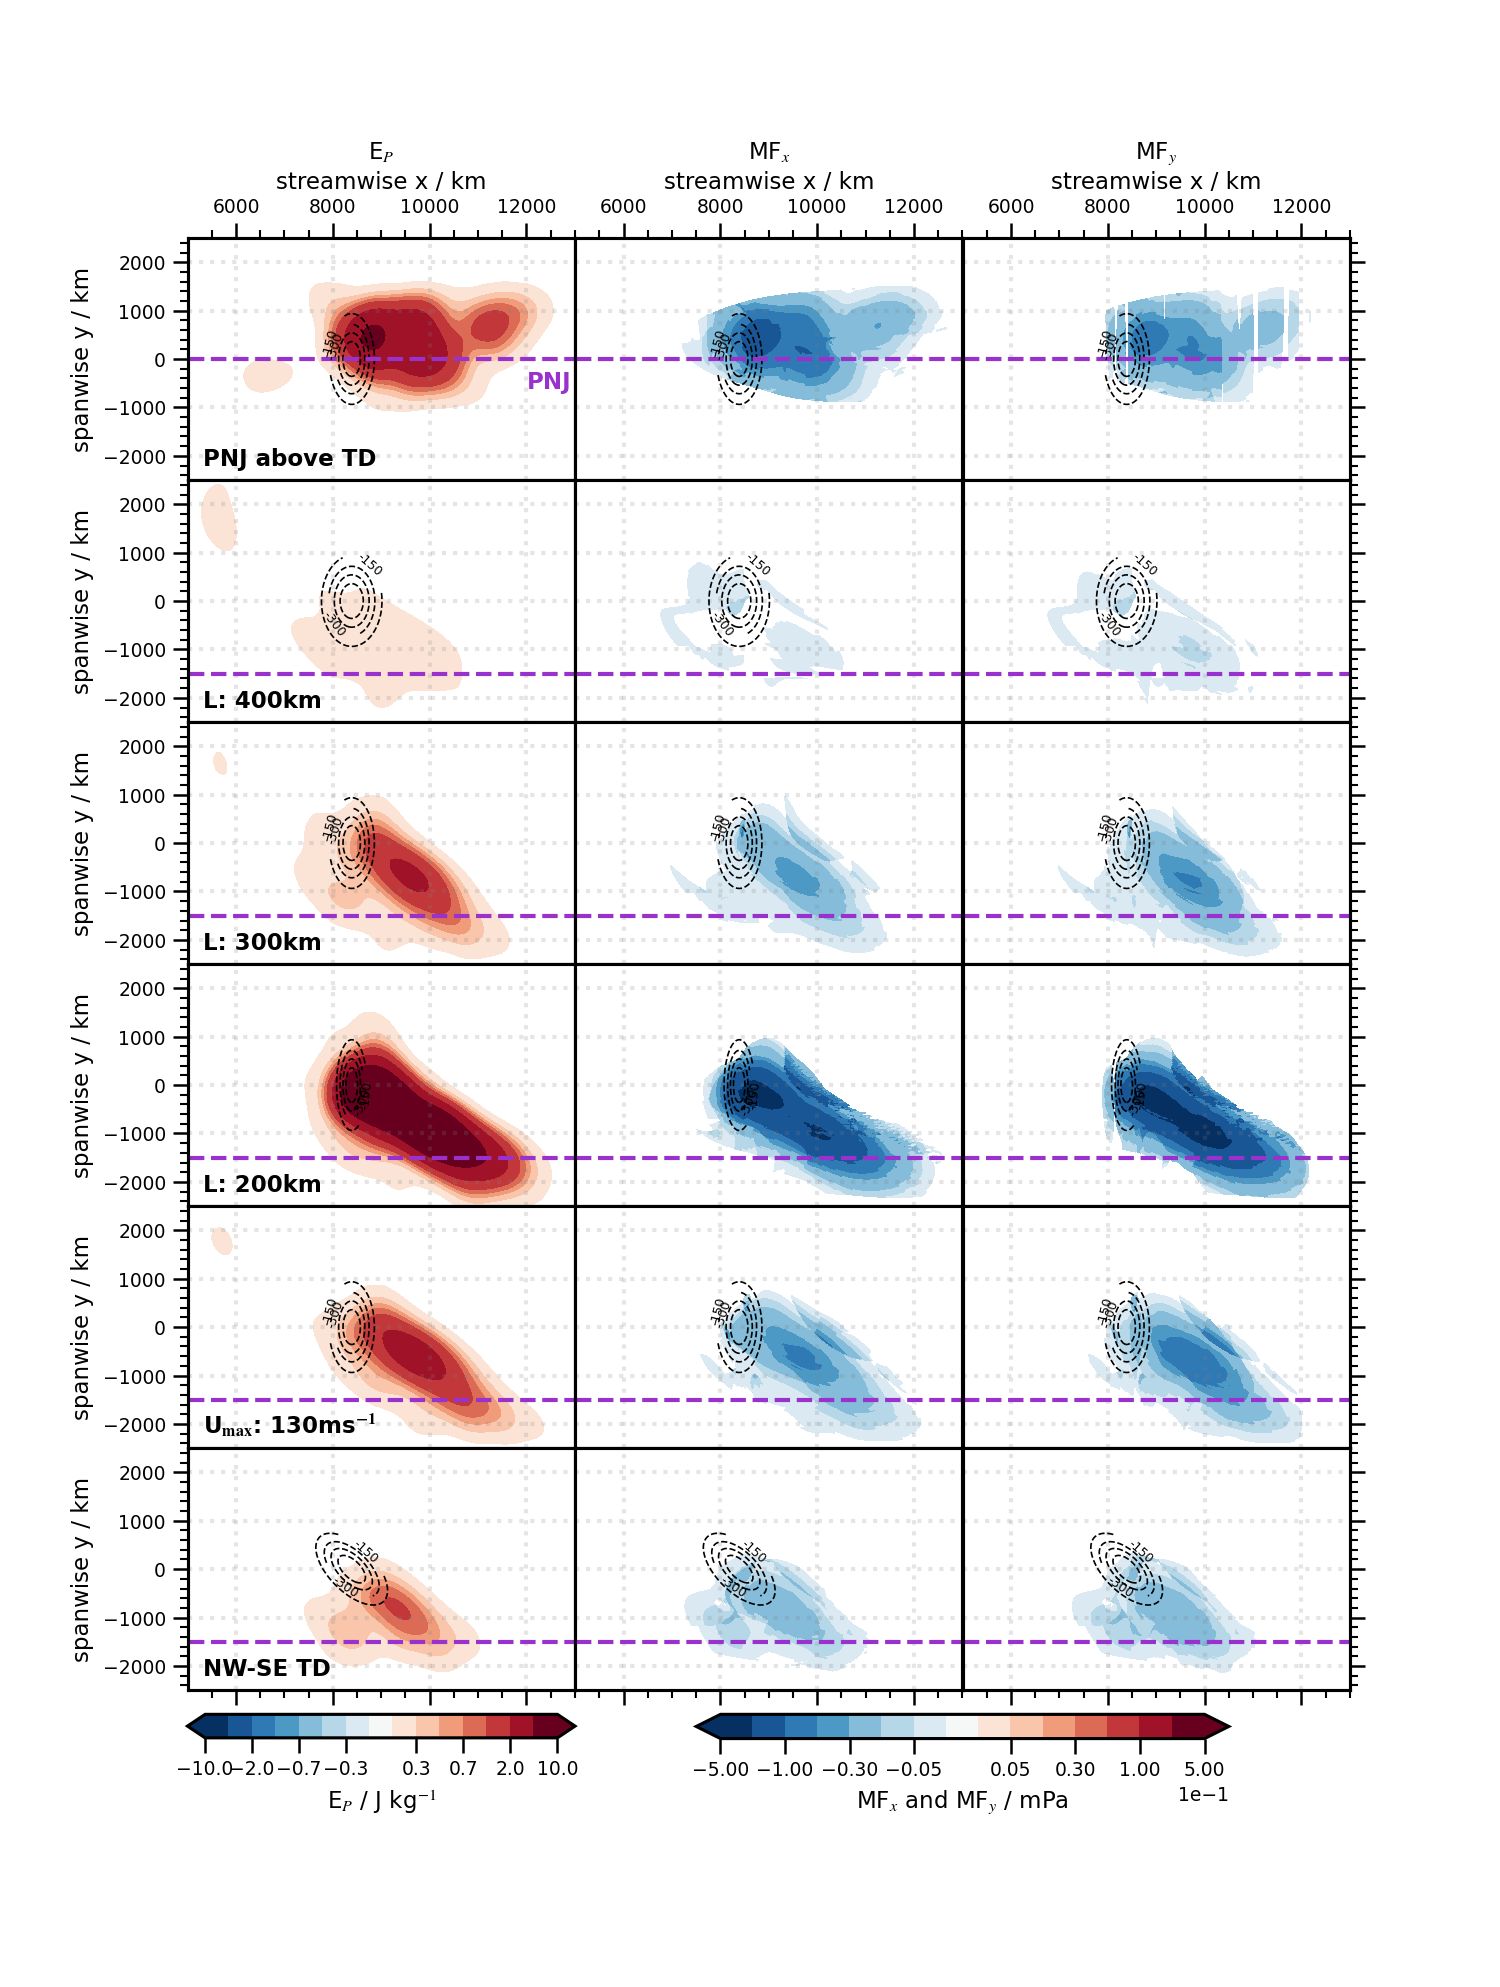
\includegraphics[width=0.99\textwidth]{figures_3D/waveletAna_fluxes_obs.png}
    \caption{Horizontal cross sections at 40km above the tropopause for five simulations with horizontal and meridional shear in a barotropic environment. Shown are $\theta$', $\lambda_x$ and $\lambda_y$ at 72h into the simulation. Dominant zonal and meridional wavelengths for each grid point are determined from wavelet analysis.}
    \label{fig:waveletAna_dudy}
\end{figure*}

\begin{figure*}[]
    \centering
    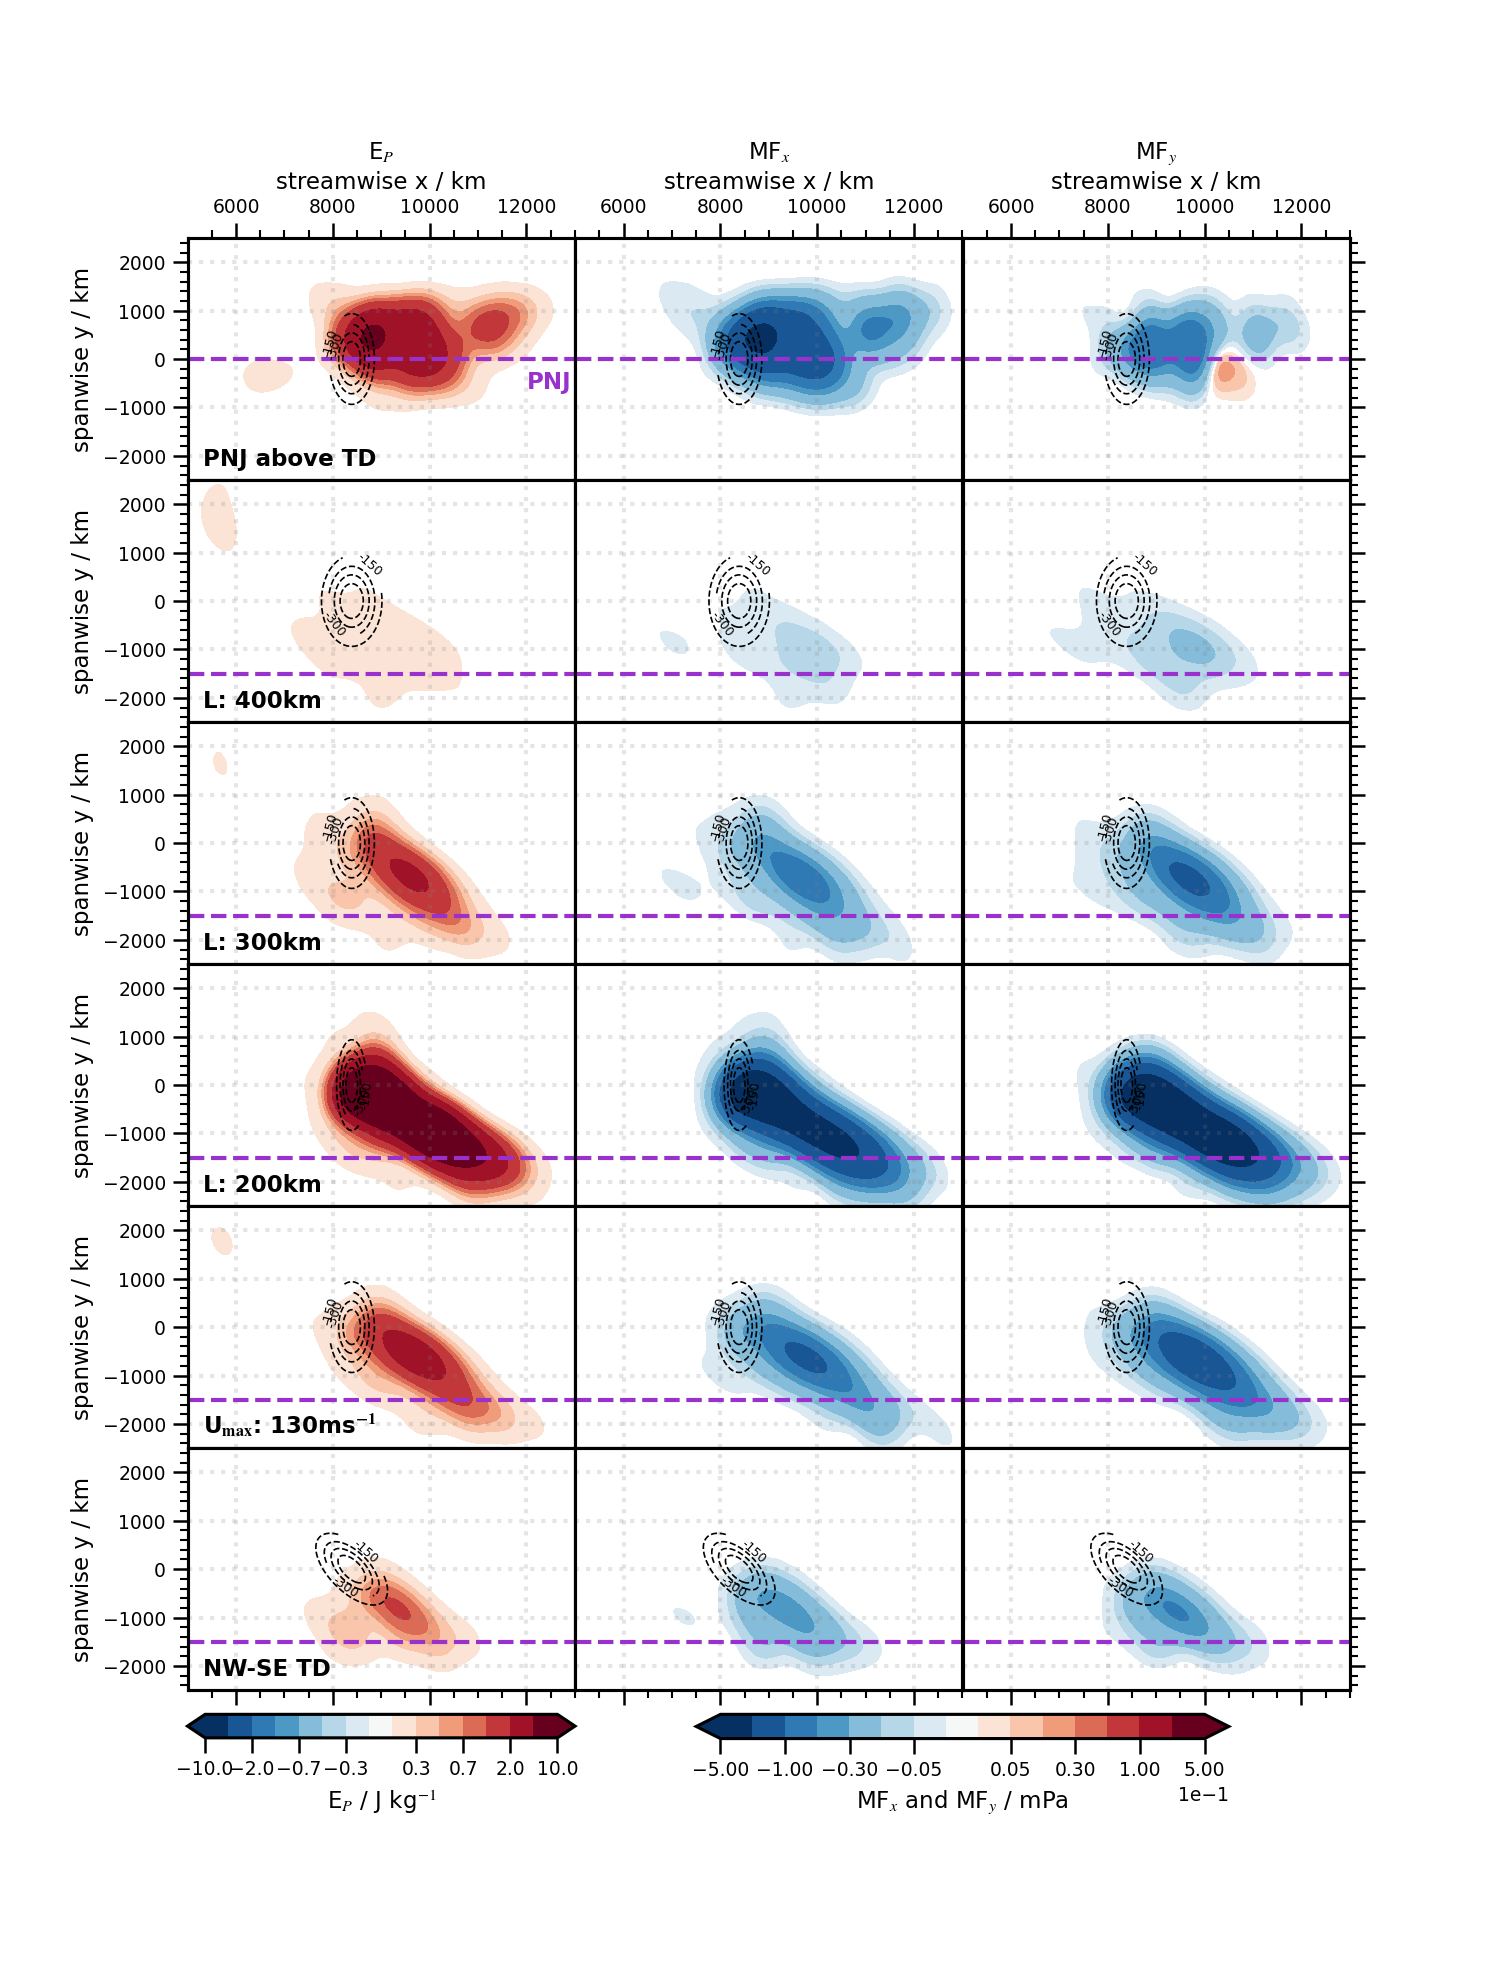
\includegraphics[width=0.99\textwidth]{figures_3D/waveletAna_fluxes_sim.png}
    \caption{Horizontal cross sections at 40km above the tropopause for five simulations with horizontal and meridional shear in a barotropic environment. Shown are $\theta$', $\lambda_x$ and $\lambda_y$ at 72h into the simulation. Dominant zonal and meridional wavelengths for each grid point are determined from wavelet analysis.}
    \label{fig:waveletAna_dudy}
\end{figure*}